The definition of adequate metrics between objects to be compared is at the
core of many machine learning methods (\emph{eg.} nearest neighbors, kernel
machines, \emph{etc.}).
When complex objects are at stake, such metrics have to be carefully designed
in order to leverage desired notions of similarity.

This section covers my works related to the definition of new metrics for
structured data such as time series or graphs.
Three tracks are investigated.
First, in Sec.~\ref{sec:kernel}, time series are seen as discrete
distributions over the feature-time product space and a kernel is defined that
efficiently compares such representations.
Second, in Sec.~\ref{sec:dtw}, time series are treated as sequences, which
means that only ordering is of importance (time delay between observations
is ignored) and variants of the Dynamic Time Warping algorithm are used.
Finally, in Sec.~\ref{sec:ot}, undirected labeled graphs are seen as
discrete distributions over the feature-structure product space and we rely on
optimal transport distances.

\section{A Temporal Kernel for Time Series}
\label{sec:kernel}

The method presented in this section consists in defining a kernel between
sets of timestamped objects (typically features).
This allows, in particular, to consider the case of irregularly sampled time
series.\footnote{This work was part of Adeline Bailly's PhD thesis.
We were co-supervising Adeline together with Laetitia Chapel.}

\subsection{Match kernel and Signature Quadratic Form Distance}

Our method relies on a kernel $k(\cdot,\cdot)$ between local
features.
Based on this local kernel, one can compute the match kernel
\cite{NIPS2009_3874} between sets of local features as:

\begin{equation}
    K(\mathbf{x}, \mathbf{x}^\prime) = \sum_i \sum_j k(x_i, x^\prime_j)
\end{equation}

\noindent
and the Signature Quadratic Form Distance (SQFD,
\cite{10.1145/1631272.1631391}) is the distance
between feature sets $\mathbf{x}$ and $\mathbf{x}^\prime$ embedded in the
Reproducing Kernel Hilbert Space (RKHS)
associated with $K$:

\begin{equation}
    SQFD(\mathbf{x}, \mathbf{x}^\prime) =
        \sqrt{K(\mathbf{x}, \mathbf{x})
              + K(\mathbf{x}^\prime, \mathbf{x}^\prime)
              - 2 K(\mathbf{x}, \mathbf{x}^\prime)}
        \, .
\end{equation}

\subsection{Local Temporal Kernel}

We introduce a time-sensitive local kernel defined as:

\begin{equation}
    k_t((x_i, t_i), (x^\prime_j, t^\prime_j)) = e^{\gamma_t (t^\prime_j - t_i)^2} k(x_i, x^\prime_j).
\end{equation}

This kernel is positive semi definite (psd), as the product of two psd kernels
and, if $k$ is the radial basis function (RBF) kernel, it can be written as:

\begin{equation}
    k_t((x_i, t_i), (x^\prime_j, t^\prime_j)) = k(g(x_i, t_i), g(x^\prime_j, t^\prime_j)).
\end{equation}
with
\begin{equation}
g(x_i, t_i) = \left( x_{i,0}, \dots , x_{i, d-1},
                            \sqrt{\frac{\gamma_t}{\gamma_f}} t_i \right)
\end{equation}

\noindent
where $x_{i,l}$ denotes the $l$-th feature of the $i$-th observation in
$\mathbf{x}$.

Figure~\ref{fig:gamma_t} illustrates the impact of the ratio
$\sqrt{\frac{\gamma_t}{\gamma_f}}$ on the kernel matrix (larger $\gamma_t$
leads to paying less attention to off-diagonal elements).

\begin{figure}[t]
    \begin{subfigure}[b]{0.3\textwidth}
         \centering
         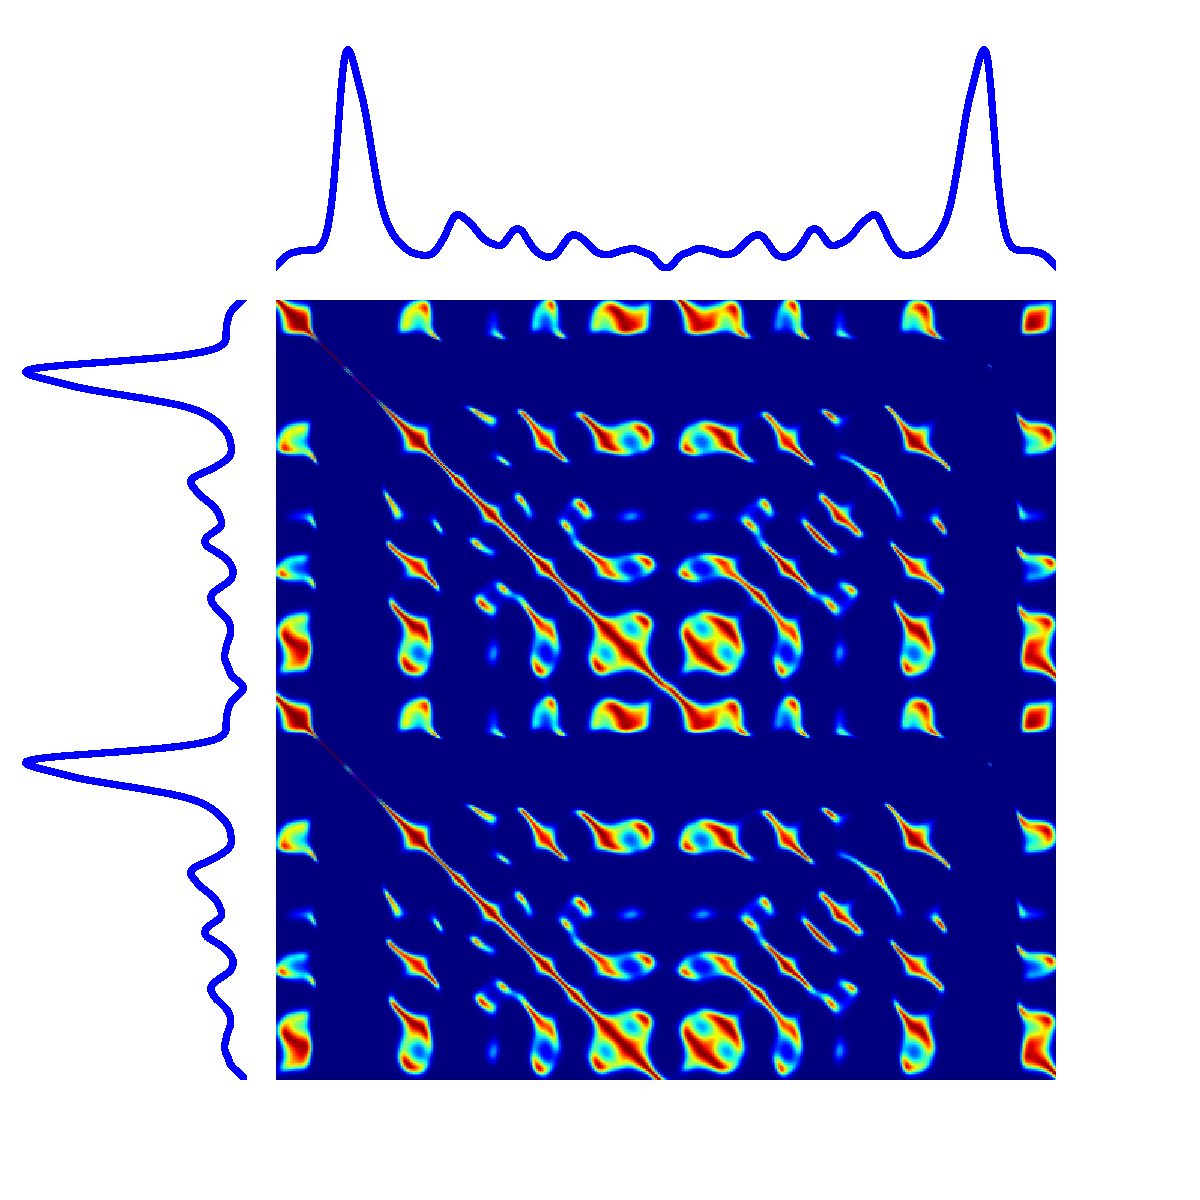
\includegraphics[width=\textwidth]{fig/gram_gammat0}
         \caption{$\gamma_t = 0$}
     \end{subfigure}
     \hfill
     \begin{subfigure}[b]{0.3\textwidth}
          \centering
          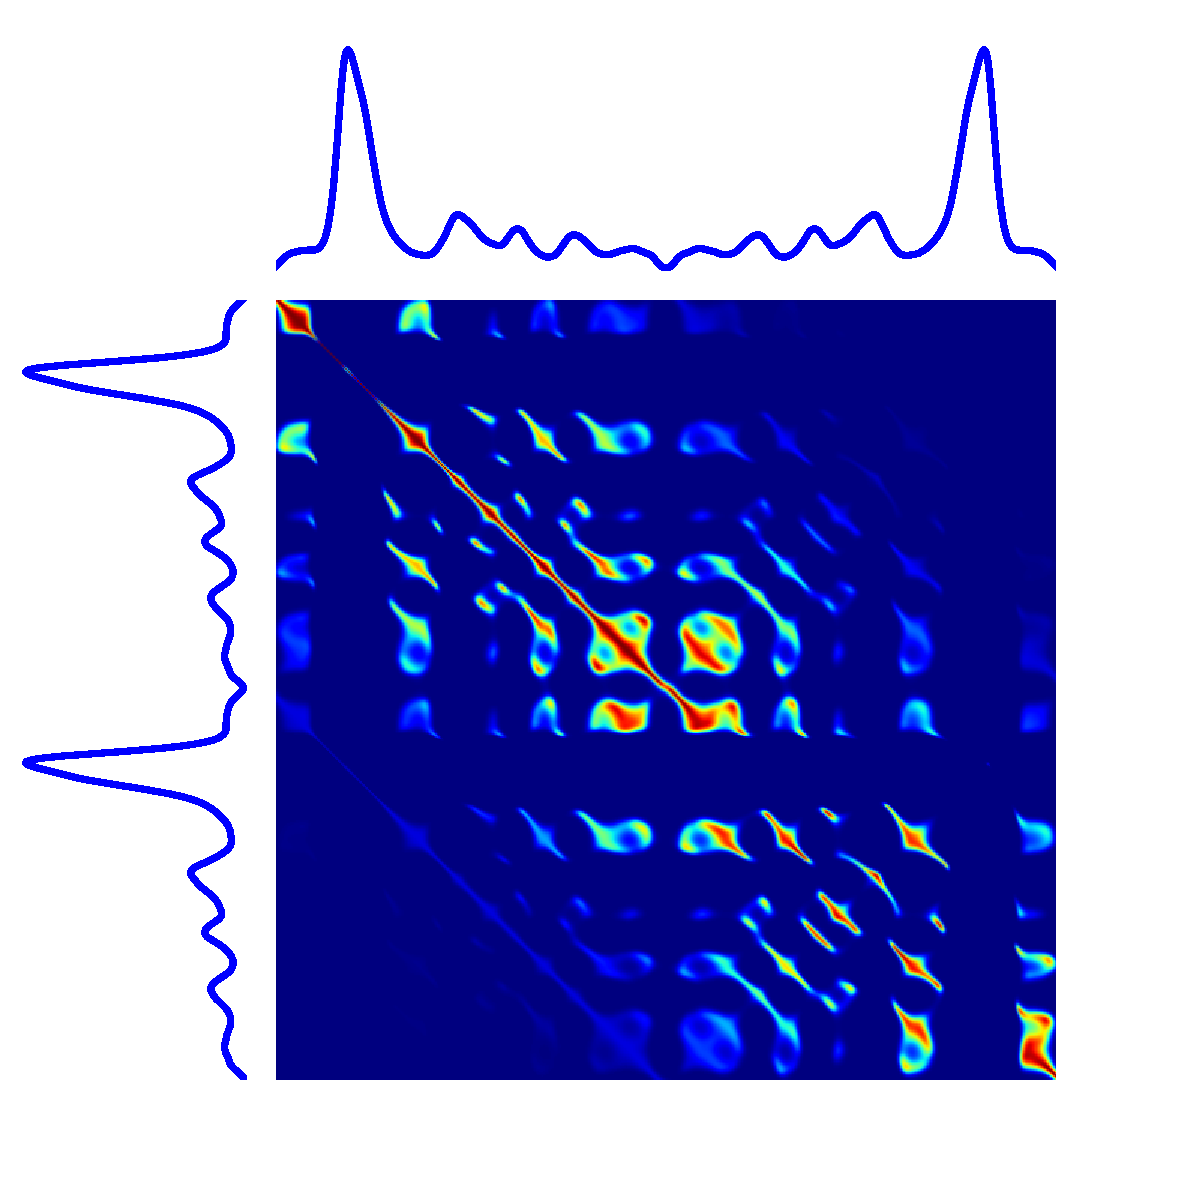
\includegraphics[width=\textwidth]{fig/gram_gammat10}
          \caption{Medium $\gamma_t$ value}
      \end{subfigure}
      \hfill
      \begin{subfigure}[b]{0.3\textwidth}
           \centering
           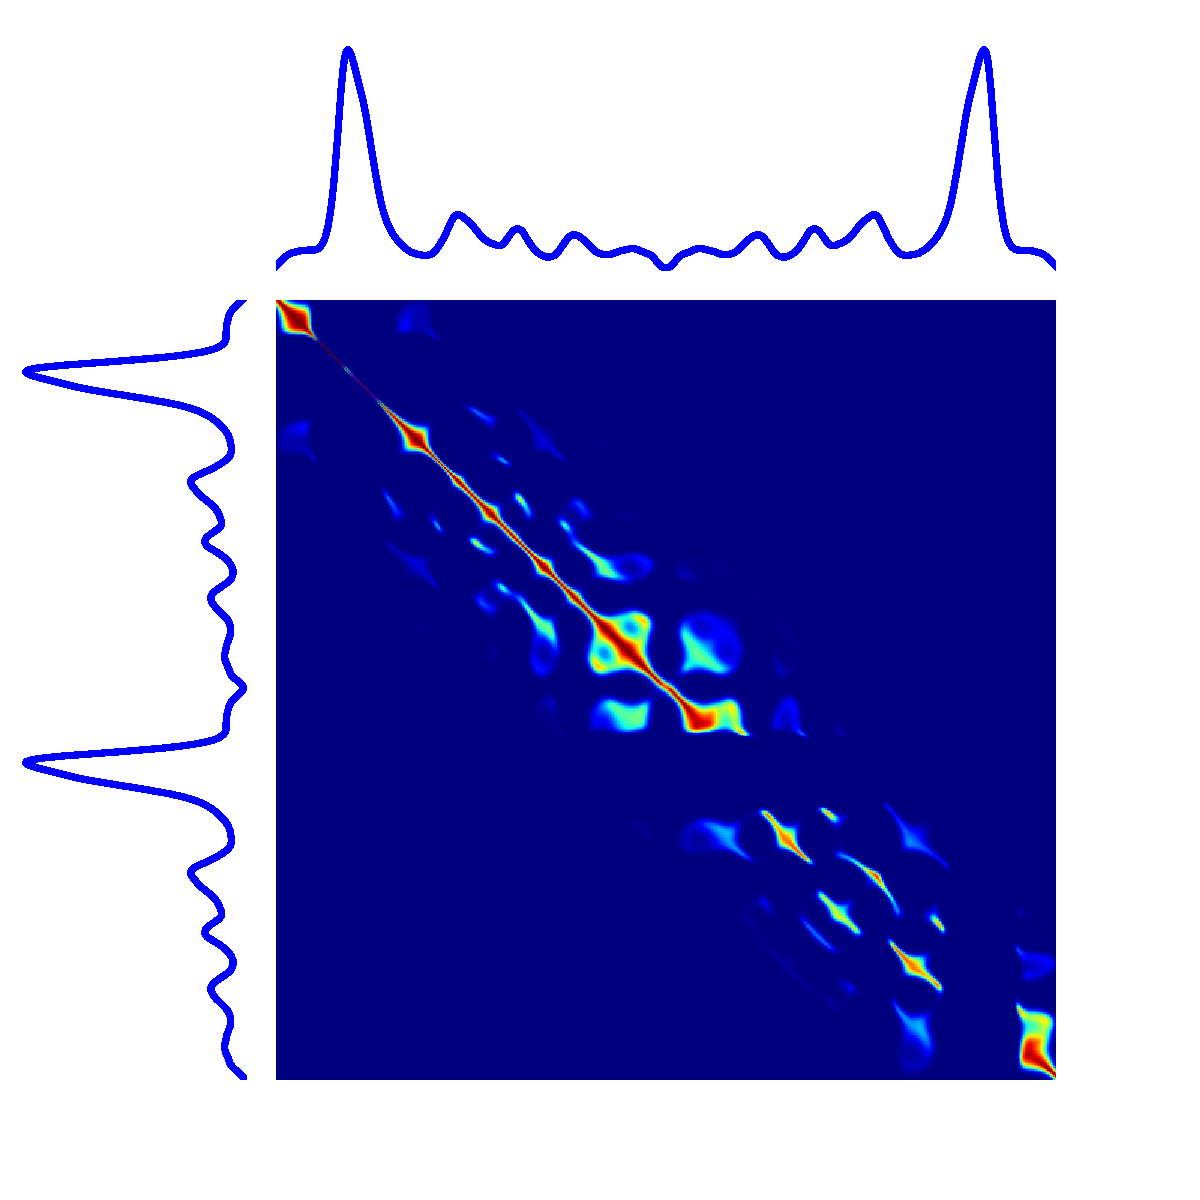
\includegraphics[width=\textwidth]{fig/gram_gammat100}
           \caption{Large $\gamma_t$ value}
       \end{subfigure}
    \caption{Effect of the $\gamma_t$ parameter on the kernel matrix on which
    SQFD relies.}
    \label{fig:gamma_t}
\end{figure}

$k_t$ is then a RBF kernel itself, and
Random Fourier Features \cite{NIPS2007_3182} can be
used in order to approximate it with a linear kernel.

If $\phi$ is a feature map such that

\begin{equation}
k_t((x_{i}, t_i), (x^\prime_j, t^\prime_j)) \approx
    \left\langle\phi(g(x_{i}, t_i)),
        \phi(g(x^\prime_{j}, t^\prime_j))\right\rangle,
\end{equation}
then

\begin{equation}
SQFD(\mathbf{x}, \mathbf{x}^\prime) \approx \left\|
    \underbrace{\frac{1}{n}\sum_i \phi(g(x_{i}, t_i))}_{b_\phi(\mathbf{x})} -
    \underbrace{\frac{1}{m}\sum_j
        \phi(g(x^\prime_{j}, t^\prime_j))}_{b_\phi(\mathbf{x}^\prime)}
    \right\|.
\end{equation}

In other words, once feature sets are embedded in this finite-dimensional
space, approximate SQFD computation is performed through (i) a barycenter
computation $b_\phi(\cdot)$ in the feature space (which can be performed
offline)
followed by (ii) a Euclidean distance computation with a time complexity of
$O(D)$, where $D$ is
the dimension of the feature map $\phi$.
Overall, we have a distance between timestamped feature sets
the precision / complexity tradeoff of which
can be tuned via the map dimensionality $D$.

\subsection{Evaluation}

In order to evaluate the method presented above, we used the UCR Time
Series Classification archive~\cite{ucr}, which, at the time, was made of
monodimensional
time series only.
We decided not to work on raw data but rather extract local features to
describe our time series.
We chose to rely on temporal SIFT features, that we had introduced in
\cite{bailly:halshs-01184900,bailly:hal-01252726}.
These features are straight-forward 1D adaptations of the Scale-Invariant
Feature Transform (SIFT) framework introduced in Computer Vision
\cite{Lowe:2004:DIF:993451.996342}.%
\footnote{Note that the use of such handcrafted features was already outdated in the
computer vision community at the time of this work.
However, in our small data context, they proved useful for the task at hand.}

We show in \cite{tavenard:halshs-01561461} that kernel approximation
leads to better trade-offs in terms of computational
complexity \emph{vs.} kernel approximation than a pre-processing of the feature sets
that would rely on $k$-means clustering.
We also show that the obtained distance, once embedded in a Support Vector
Machine with Gaussian kernel, leads to classification performance that is
competitive with the state-of-the-art.

\section{Dynamic Time Warping}
\label{sec:dtw}

This section covers works related to Dynamic Time Warping for time series.

\subsection{Definition}


Dynamic Time Warping (DTW,~\cite{sakoe1978dynamic}) is a similarity measure
between time series.
Let us consider two time series $\mathbf{x}$ and
$\mathbf{x}^\prime$ of respective lengths $n$ and
$m$.
Here, all elements $x_i$ and $x^\prime_j$ are assumed to lie in the same
$p$-dimensional space and the exact timestamps at which observations occur are
considered uninformative: only their ordering matters.

\subsubsection{Optimization problem}

DTW between $\mathbf{x}$ and $\mathbf{x}^\prime$ is formulated as the following
optimization problem:

\begin{equation}
DTW(\mathbf{x}, \mathbf{x}^\prime) =
    \min_{\pi \in \mathcal{A}(\mathbf{x}, \mathbf{x}^\prime)}
        \sqrt{ \sum_{(i, j) \in \pi} d(x_i, x^\prime_j)^2 }
\label{eq:dtw}
\end{equation}

where $\mathcal{A}(\mathbf{x}, \mathbf{x}^\prime)$ is the set of all admissible
paths, \emph{ie.} the set of paths $\pi$ such that:

\begin{itemize}
\item $\pi$ is a list $[\pi_0, \dots , \pi_{K-1}]$ of index pairs
  $\pi_k = (i_k, j_k)$ with $0 \leq i_k < n$ and $0 \leq j_k < m$
\item $\pi_0 = (0, 0)$ and $\pi_{K-1} = (n - 1, m - 1)$
\item for all $k > 0$ , $\pi_k = (i_k, j_k)$ is related to
  $\pi_{k-1} = (i_{k-1}, j_{k-1})$ as follows:
  \begin{itemize}
  \item $i_{k-1} \leq i_k \leq i_{k-1} + 1$
  \item $j_{k-1} \leq j_k \leq j_{k-1} + 1$
\end{itemize}
\end{itemize}

Here, a path can be seen as a temporal alignment of time series and the optimal
path (as presented in Figure~\ref{fig:dtw}) is such that
Euclidean distance between aligned (\emph{ie.} resampled) time series is
minimal.

\begin{figure}[t]
\centering
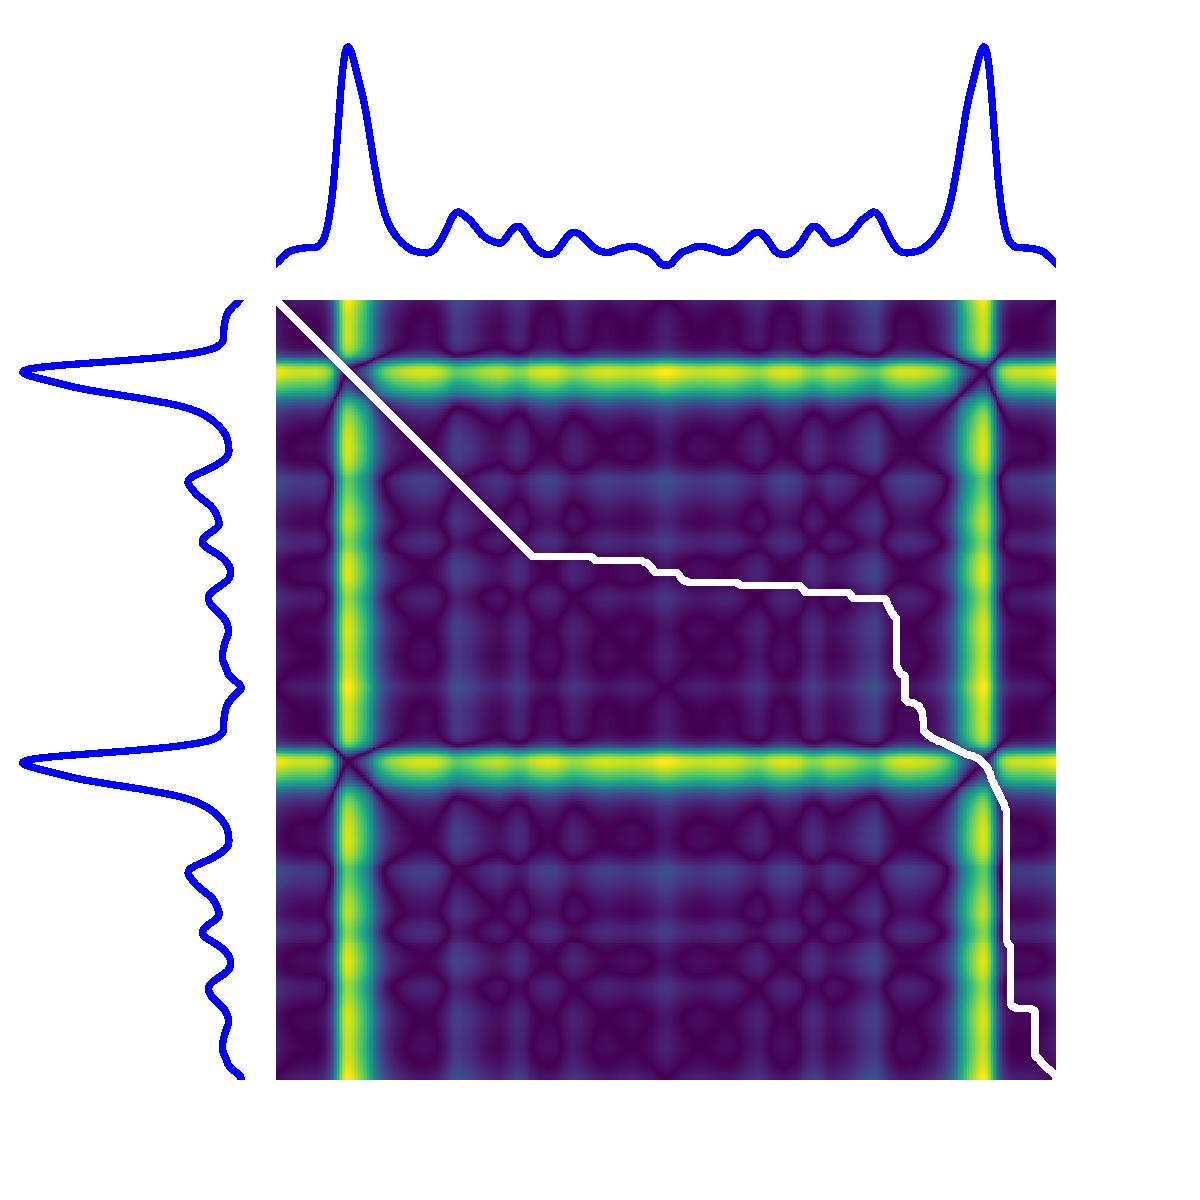
\includegraphics[width=.4\textwidth]{fig/dtw}
\caption{DTW path (in white) for a given pair of time
series, shown on top of the cross-similarity matrix that stores
$d(x_i, {x}^\prime_j)$
values. \label{fig:dtw}}
\end{figure}

\subsubsection{Algorithmic solution}

There exists an $O(mn)$ algorithm to compute the exact optimum for this
problem (see Algorithm~\ref{algo:dtw}).

\begin{algorithm}[t]
 \caption{DTW algorithm. Note that, for the sake of simplicity, out-of-bounds accesses to $C$ are supposed to return $\infty$ as a value.}
 \label{algo:dtw}
 \KwData{$(\mathbf{x}, \mathbf{x}^\prime)$ : a pair of time series}
 \For{$i$ = 0..$n-1$}{
   \For{$j$ = 0..$m-1$}{
     dist = $d(x_i, x^\prime_j)^2$ \\
       \eIf{$i$ == 0 and $j$ == 0}{
         $C_{i, j} = dist$
       }{
         $C_{i, j} = dist + \min(C_{i-1, j}, C_{i, j-1}, C_{i-1, j-1})$
       }
    }
  }
  \Return $\sqrt{C_{n - 1, m - 1}}$
\end{algorithm}


\subsubsection{Properties}

Dynamic Time Warping holds the following properties:

\begin{itemize}
\item $\forall \mathbf{x}, \mathbf{x}^\prime, DTW(\mathbf{x}, \mathbf{x}^\prime) \geq 0$
\item $\forall \mathbf{x}, DTW(\mathbf{x}, \mathbf{x}) = 0$
\end{itemize}

However, mathematically speaking, DTW is not a valid metric since it does
not satisfy the triangular inequality nor the identity of indiscernibles.

\subsubsection{Setting additional constraints}

The set of temporal deformations to which DTW is invariant can be reduced by
setting additional constraints on the set of acceptable paths.
These constraints typically consist in forcing paths to lie close to the
diagonal.

First, the Sakoe-Chiba band is parametrized by a radius $r$ (number of
off-diagonal elements to consider, also called warping window size sometimes),
as illustrated in Figure~\ref{fig:sakoe}.

Second, the Itakura parallelogram sets a maximum slope $s$ for alignment
paths, which leads to a parallelogram-shaped constraint (see Figure~\ref{fig:itakura}).

\begin{figure}[t]
    \begin{subfigure}[b]{0.4\textwidth}
         \centering
         
\includegraphics[width=\textwidth]{fig/sakoe}
         \caption{Sakoe-Chiba band of radius $r=3$}
         \label{fig:sakoe}
     \end{subfigure}
     \hfill
     \begin{subfigure}[b]{0.4\textwidth}
          \centering
          
\includegraphics[width=\textwidth]{fig/itakura}
          \caption{Itakura parallelogram of maximum slope $s=2$}
          \label{fig:itakura}
      \end{subfigure}
    \caption{Global constraints for Dynamic Time Warping.}
\end{figure}

\subsection{Constrained Dynamic Time Warping}

In this section, we present a method to regularize Dynamic Time Warping
by setting constraints on the length of the admissible warping
paths~\cite{zhang2017dynamic}.%
\footnote{This work is a part of Zheng Zhang's PhD thesis. It was performed
during Zheng's stay at LETG in 2015-2016.
I was not directly involved in the supervision Zheng's PhD thesis.}

\subsubsection{Formulation and Optimization}

As discussed above, a common way
to restrict the set of admissible temporal distortions for Dynamic Time Warping
consists in forcing paths to stay close to the diagonal through the use of
Sakoe-Chiba band or Itakura parallelogram constraints.
A limitation of these global constraints is that they completely
discard some regions of the alignment matrix \emph{a priori}
(\emph{i.e.} regardless of the involved data).

To alleviate this limitation, we propose Limited warping path length DTW (LDTW)
that adds a path length constraint to the DTW
optimization problem such that a path is said admissible for our method iff:

\begin{itemize}
\item it is an admissible DTW path;
\item its length $K$ is lower or equal to a user-defined bound $K_\text{max}$.
\end{itemize}

We have proposed an algorithm that stores, at each step $(i, j)$, optimal
alignment scores for all admissible alignment path lengths.
This gives the general LDTW algorithm presented in Algorithm~\ref{algo:ldtw}.

\begin{algorithm}[t]
 \caption{LDTW algorithm. For the sake of simplicity, out-of-bounds accesses to $C$ are assumed to return $\infty$.}
 \label{algo:ldtw}
 \KwData{$(\mathbf{x}, \mathbf{x}^\prime)$ : a pair of time series, $K_\text{max}$: an upper bound on the path length}
 \For{$i$ = 0..$n-1$}{
   \For{$j$ = 0..$m-1$}{
     \texttt{// Set infinite cost for non-admissible lengths:} \\
     $C_{i, j, :} = (\infty, \cdots , \infty)$ \\
     dist = $d(x_i, x^\prime_j)^2$ \\
     \texttt{// The core difference with DTW is the following loop:} \\
     \For{$l \in \mathrm{admissible\_lengths}(i, j, K_\text{max})$}{
       \eIf{$i$ == 0 \textup{\textbf{and}} $j$ == 0}{
         $C_{i, j, l} = dist$
       }{
         $C_{i, j, l} = dist + \min(C_{i-1, j, l-1}, C_{i, j-1, l-1}, C_{i-1, j-1, l-1})$
       }
 	  }
    }
  }
  \Return $\sqrt{\min_{k} C_{n - 1, m - 1, k}}$
\end{algorithm}


The question is then to compute the set
\texttt{admissible\_lengths}$(i, j, K_\text{max})$.
We have shown that this set can be computed explicitly and that its cardinal
is $O(\min(i, j))$.
Overall, we have a $O(mn^2 + nm^2)$ complexity for this exact algorithm.

\subsubsection{Empirical Observations}

First, one can see in Figure~\ref{fig:ldtw} that the resulting alignments
effectively limits the number of singularities in the obtained alignments as
compared to DTW.

\begin{figure}[t]
    \begin{subfigure}[b]{\textwidth}
         \centering
         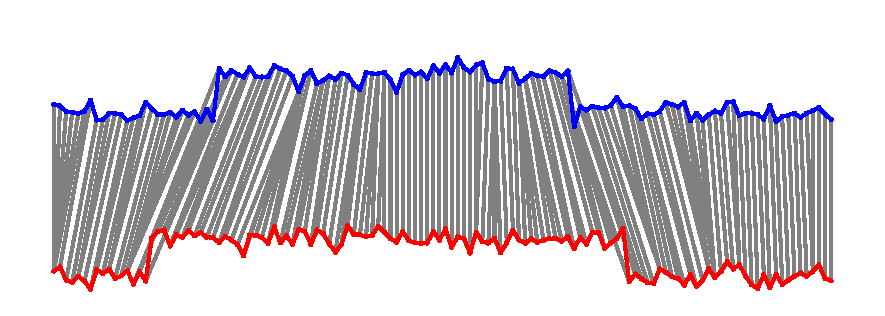
\includegraphics[width=.8\textwidth]{fig/dtw_warping_length}
         \caption{LDTW matches}
     \end{subfigure}
     \begin{subfigure}[b]{\textwidth}
          \centering
          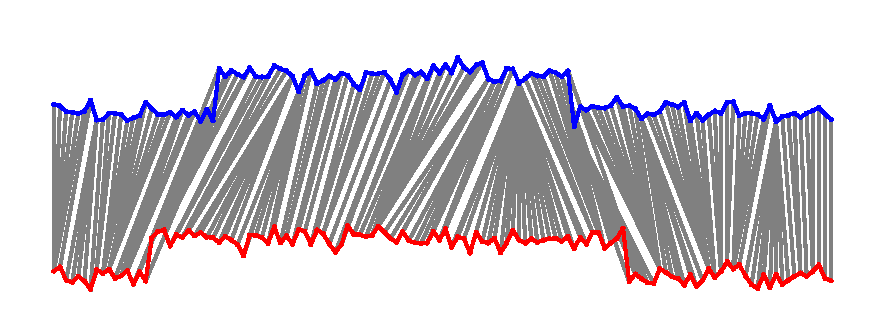
\includegraphics[width=.8\textwidth]{fig/dtw_warping_length_b}
          \caption{DTW matches}
      \end{subfigure}
    \caption{Compared matches obtained with DTW and its
    warping-length-constrained variant LDTW. Note the comparatively smaller
    temporal distortions induced by LDTW.}
    \label{fig:ldtw}
\end{figure}

Moreover, our experiments on UCR Time Series Datasets~\cite{ucr} show that
this similarity measure, when used in a 1-Nearest Neighbor Classifier, leads to
a higher accuracy than other constrained DTW variants
(Sakoe-Chiba band and Itakura parallelogram).

\subsection{DTW Alignment as an Adaptive Resampling Strategy}

In this section, we present a method that uses Dynamic Time Warping (DTW)
on multimodal time series, \emph{i.e.} time series that are made of several
features recorded over time.
The method relies on the assumption that one of the considered modalities
(called
reference modality in the following) can be used as a reference to (temporally)
realign other modalities~\cite{dupas:halshs-01228397}.
It has been used in the context of hydrological measurements to align pollutant
concentration profiles based on discharge time series.%
\footnote{This work is a part of Rémi Dupas' PhD thesis (in Environment
Sciences).
I was not directly involved in the supervision of Rémi's PhD thesis.}

This approach can be seen as the DTW counterpart of other works that rely on
Optimal Transport for Domain Adaptation~\cite{courty:hal-02112785}.
One significant difference, however, is that it relies on a reference modality
for
alignment.
This design choice is guided by our application context.

\subsubsection{Motivating Use Case}

Phosphorus (P) transfer during storm events represents a significant part of
annual P loads in streams and contributes to eutrophication in downstream water
bodies. To improve understanding of P storm dynamics, automated or
semi-automated methods are needed to extract meaningful information from
ever-growing water quality measurement datasets.

Clustering techniques have proven useful for identifying seasonal storm
patterns and thus for increasing knowledge about seasonal variability in storm
export mechanisms (\emph{e.g.},~\cite{aubert:halshs-00906292}).
Clustering techniques usually require calculating distances between pairs of
comparable points in multiple time series. For this reason, direct clustering
(without using hysteresis-descriptor variables) of high-frequency storm
concentration time series is usually irrelevant because the lengths of recorded
time series (number of
measurement points) might differ and/or measurement points may have different
positions relative to the hydrograph (flow rise and recession); hence, it is
difficult to calculate a distance between pairs of comparable points.

The aim of this study was to develop a clustering method that overcomes this
limit and test its ability to compare seasonal variability of P storm dynamics
in two headwater watersheds. Both watersheds are ca. 5 km$^2$, have similar
climate and geology, but differ in land use and P pressure intensity.

\subsubsection{Alignment-based Resampling Method}

In the above-described setting, we have access to one modality (discharge,
commonly denoted $Q$) that is representative of the evolution of the flood.
Temporal realignment based on this modality allows to overcome three
difficulties that can arise when comparing storm-event data.
Indeed, time series can have

\begin{enumerate}
\item different starting times due to the discharge threshold at which the
samplers were triggered,
\item different lengths, and
\item differences in phase that yield different temporal localizations of the
discharge peak.
\end{enumerate}

To align time series, we use the path associated with DTW.
This matching path can be viewed as the optimal way to perform point-wise
alignment of time series.

For each discharge time series $\mathbf{x}^{(i)}_\text{Q}$, we compute the
matching path $\pi_\text{Q}$ and use it to find the optimal alignment wrt.
the same reference discharge time series $\mathbf{x}^\text{ref}_\text{Q}$.
The reference discharge time series used in this study is chosen
as a storm event with full coverage of flow rise and flow recession phases.
Alternatively, one could choose a synthetic idealized storm hydrograph.

We then use barycentric mapping based on the obtained matches to realign other
modalities to the timestamps of the reference time series, as shown in
Figure~\ref{fig:dtw_da}.

\begin{figure}[t]
    \begin{subfigure}[b]{\textwidth}
         \centering
         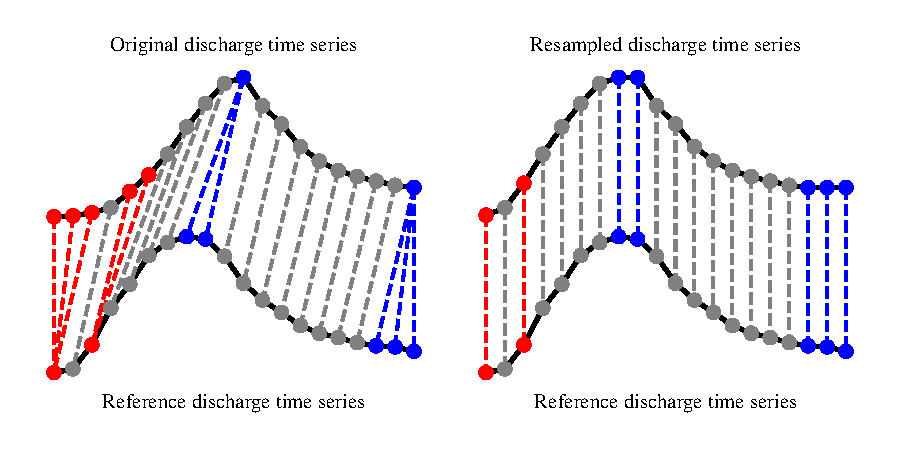
\includegraphics[width=.7\textwidth]{fig/dtw_da}
     \end{subfigure}
      \begin{subfigure}[b]{\textwidth}
           \centering
           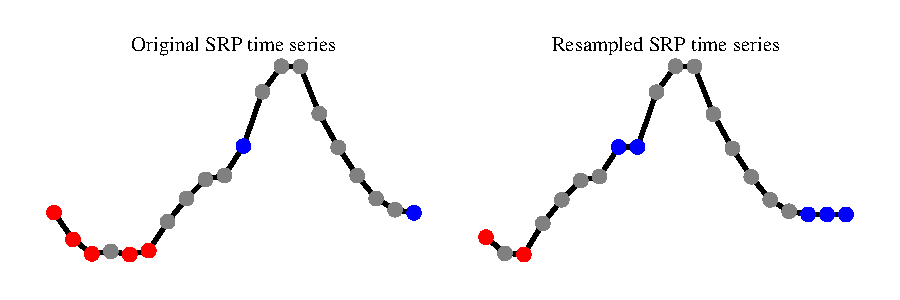
\includegraphics[width=.7\textwidth]{fig/dtw_da_b}
       \end{subfigure}
    \caption{Adaptive resampling strategy. Top row: A discharge time series is
    resampled so that its timestamps match those of a reference one. Bottom row:
    The same temporal transformation is applied to all other modalities
    (\emph{e.g.} SRP concentration) of the given sample.}
    \label{fig:dtw_da}
\end{figure}

At this point, each time series is transformed to series of $n$
$p$-dimensional measurements, where $n$ is the length of the
reference discharge time series and $p$ is the number of water quality
parameters considered in the study (\emph{i.e.} all modalities except the
discharge).
In a second step, a standard $k$-means algorithm is used to cluster
realigned time series.
Note that a Euclidean distance can be used for clustering since time series
have already been temporally realigned; hence, time-sensitive metrics (such as
DTW) are no longer needed.

This method proved useful to extract meaningful clusters and an \emph{a posteriori}
analysis of the clusters enabled to identify the export dynamics of pollutants
in different geographical areas of the study sites, which then led to management
recommendations, as detailed in~\cite{dupas:halshs-01228397}.

\subsection{DTW with Global Invariances}
\label{sec:dtw_gi}

In this work we address the problem of comparing time series while taking
into account both feature space transformation and temporal variability.
The proposed framework combines a latent global transformation of the feature
space with the widely used Dynamic Time Warping (DTW).
This work is available as preprint~\cite{vayer2020time}.%
\footnote{This work is part of Titouan Vayer's PhD thesis.
We are co-supervising Titouan together with Laetitia Chapel and Nicolas Courty.}

\subsubsection{Definition}

Let $\mathbf{x}$ and $\mathbf{x^\prime}$ be two time series of respective
lengths $n$ and $m$.
Here, features from both time series are not assumed to lie in the same ambient
space, but it is assumed that features from $\mathbf{x}$ lie in $\mathbb{R}^p$
while features from $\mathbf{x^\prime}$ lie in $\mathbb{R}^{p'}$
In the following, we assume $p \geq p'$ without loss of generality.
In order to allow comparison between time series $\mathbf{x}$ and
$\mathbf{x^\prime}$,
we will optimize on a family of functions $\mathcal{F}$ that map features from
$\mathbf{x^\prime}$ onto the feature space in which features from $\mathbf{x}$
lie. More formally, we define Dynamic Time Warping with Global Invariances
(DTW-GI) as the solution of the following joint optimization problem:

\begin{equation}
    \text{DTW-GI}(\mathbf{x}, \mathbf{x^\prime}) =
        \min_{f \in \mathcal{F}, \pi \in \mathcal{A}(\mathbf{x}, \mathbf{x^\prime})}
            \sqrt{ \sum_{(i, j) \in \pi} d(x_i, f(x^\prime_j))^2 } \, ,
    \label{eq:dtwgi}
\end{equation}

where $\mathcal{F}$ is a family of functions from $\mathbb{R}^{p^\prime}$ to
$\mathbb{R}^{p}$.

This similarity measure estimates both temporal alignment and feature space
transformation between time series simultaneously, allowing the alignment of
time series when the similarity should be defined up to a global transformation.
Time series do not have to lie in the same ambient space, as presented in
Figure~\ref{fig:dtw-gi}.

\begin{figure}[t]
    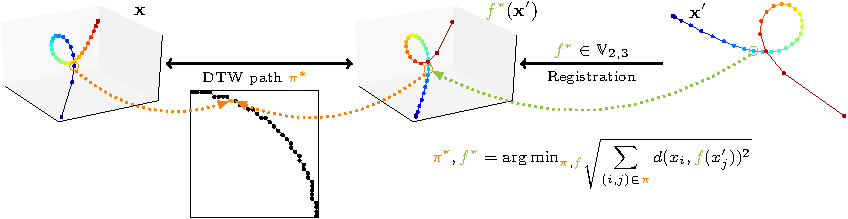
\includegraphics[width=\linewidth]{fig/dtw_gi_cropped}
    \caption{DTW-GI aligns time series by optimizing on temporal alignment
    (through Dynamic Time Warping) and feature space transformation (denoted
    $f$ here). Time series represented here are color-coded trajectories, whose
    starting (resp. end) point is depicted in blue (resp. red).}
    \label{fig:dtw-gi}
\end{figure}



\subsubsection{Optimization}

Optimization of the quantity in Equation \eqref{eq:dtwgi} can be performed
\emph{via} Block Coordinate Descent.
In a nutshell, optimization alternates between the following two steps:

1. for a fixed $f$, determine the optimal alignment path $\pi$ using the DTW
algorithm;
2. for a fixed path $\pi$, the optimal map $f$ (when $\mathcal{F}$ is the
Stiefel manifold) is obtained through Singular Value Decomposition.

Interestingly, this optimization strategy where we alternate between time
series alignment, \emph{i.e.} time correspondences between both time series, and
feature space transform optimization can be seen as a variant of the Iterative
Closest Point (ICP) method in image registration~\cite{CHEN1992145}, in
which  nearest neighbors are replaced by matches resulting from DTW alignment.

We also introduce soft counterparts following the definition of softDTW
from~\cite{cuturi2017soft}.
In this case, optimization consists in gradient descent and a wider variety of
feature space transformation families can be considered.

\begin{figure}[t]
	\centering
	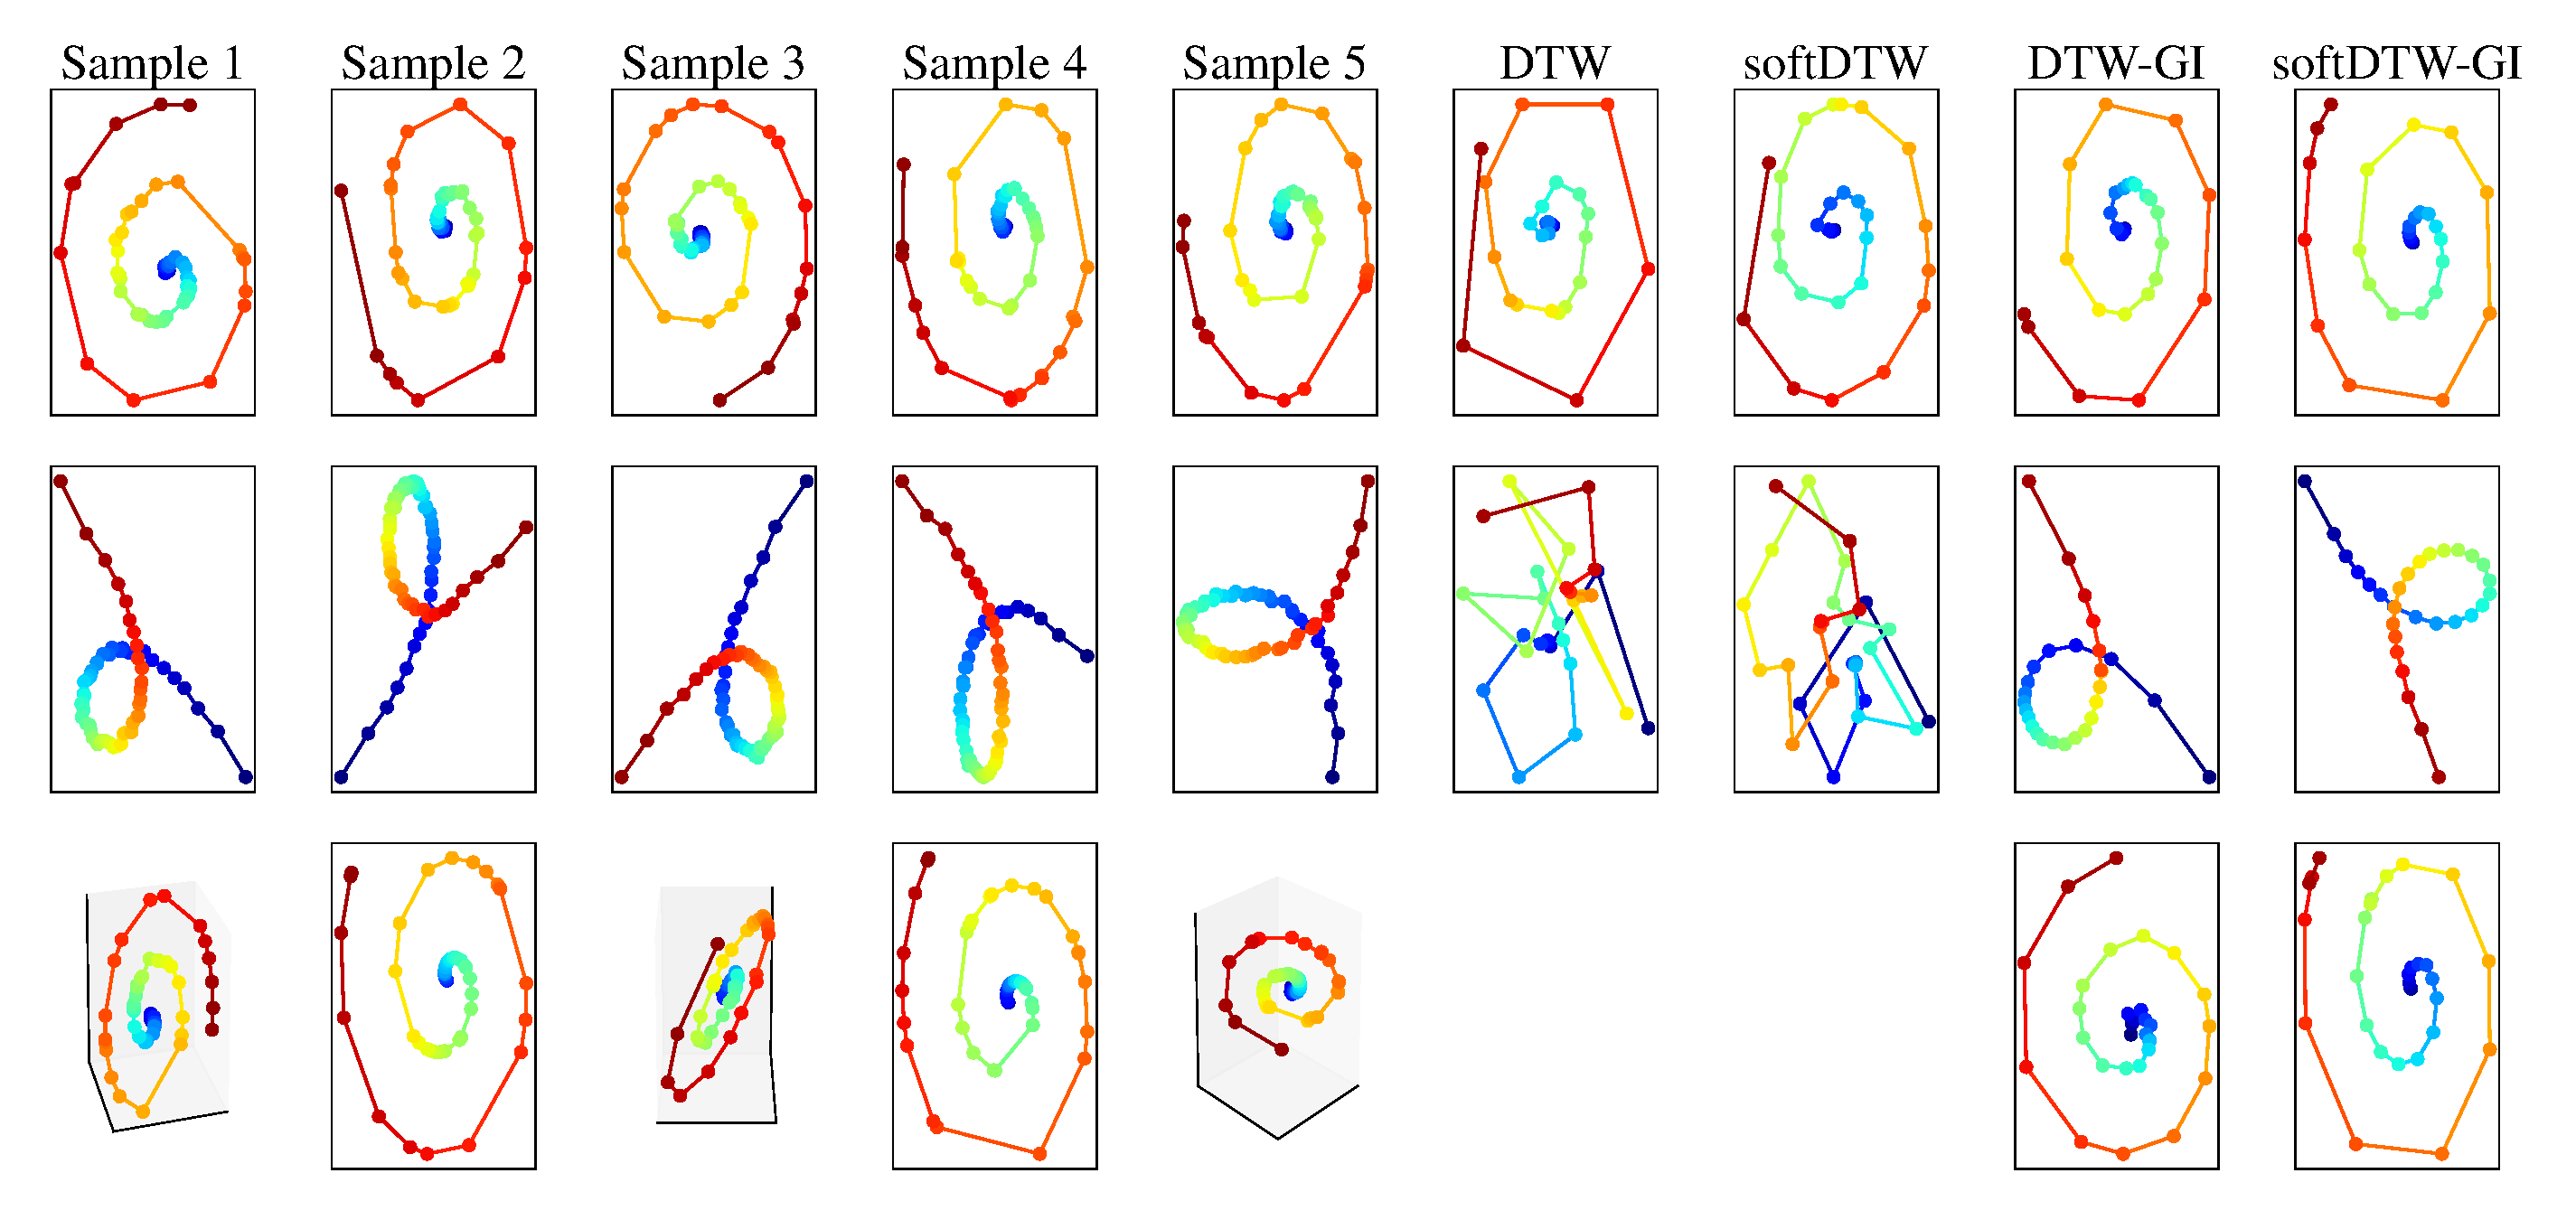
\includegraphics[width=\linewidth]{fig/barycenter_toys_allinone}
	\caption{
		Barycenter computation using (i) DTW and softDTW baseline approaches, (ii) their rotation-invariant counterparts DTW-GI and soft-DTW-GI.
		Each row correspond to a different dataset, and the latter one contains both 2d and 3d trajectories, hence cannot be tackled by any baseline method.
		Trajectories are color-coded from blue (beginning of the series) to red (end of the series).
		\label{fig:dtw_gi_bary}
	}
\end{figure}

Figure~\ref{fig:dtw_gi_bary} presents examples of barycenters obtained with
various DTW-based barycenter computation methods to illustrate the interest of
our approach.
We validate the utility of these similarity measures on real world
datasets on the tasks of human motion prediction (where motion is captured under
different points of view) and cover song identification (where song similarity
is defined up to a key transposition).
In both these settings, we observe that joint optimization on feature space
transformation and temporal alignment improves over standard approaches that
consider these as two independent steps.


\section{Optimal Transport for Structured Data}
\label{sec:ot}

This section covers my works related to Optimal Transport distances for
structured data such as graphs.
In order to compare graphs, we have introduced the Fused Gromov Wasserstein
distance that interpolates between Wasserstein distance between node feature
distributions and Gromov-Wasserstein distance between structures.%
\footnote{This work is part of Titouan Vayer's PhD thesis.
We are co-supervising Titouan together with Laetitia Chapel and Nicolas Courty.}

Here, we first introduce both Wasserstein and Gromov-Wasserstein distances and
some of our results concerning computational considerations related to the
latter.

\subsection{Wasserstein and Gromov-Wasserstein distances}

Let $\mu = \sum_i h_i \delta_{x_i}$ and $\mu' = \sum_i h^\prime_i \delta_{x^\prime_i}$
be two
discrete distributions lying in the same metric space $(\Omega, d)$.
Then, the $p$-Wasserstein distance is defined as:

\begin{equation}
    W_p(\mu, \mu') = \min_{\pi \in \Pi(\mu, \mu^\prime)}
        \left(\sum_{i,j} d(x_i, x^\prime_j)^p \pi_{i,j} \right)^{\frac{1}{p}}
    \label{eq:wass}
\end{equation}

where $\Pi(\mu, \mu^\prime)$ is the set of all admissible couplings between
$\mu$ and $\mu'$ (\emph{ie.} the set of all matrices with marginals $h$ and $h'$).%
\footnote{Note that the 2-Wasserstein distance is very similar in its formulation to
the Dynamic Time Warping similarity presented in Sec.~\ref{sec:dtw}.
The only difference lies in the constraints that are enforced in the
optimization problems.
For Wasserstein, a coupling needs to meet marginal constraints to be considered
valid while for Dynamic Time Warping, a path shall (i) not break the order of
the sequences at stake and (ii) enforce alignment of complete series (from
beginning to end).}

This distance is illustrated in Figure~\ref{fig:wass}.

\begin{figure}
\centering
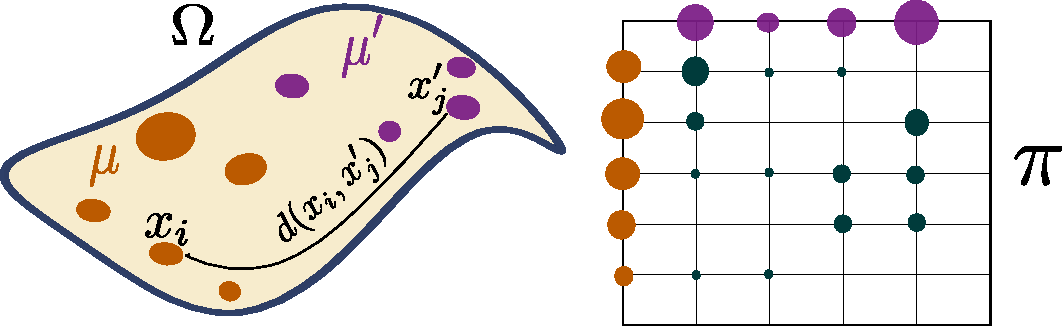
\includegraphics[width=.6\textwidth]{fig/wass}
\caption{Wasserstein distance. \label{fig:wass}}
\end{figure}

When distributions $\mu$ and $\mu'$ do not lie in the same ambient space,
however, one cannot compute their Wasserstein distance. An alternative that was
introduced in~\cite{memoli2011gromov} relies on matching intra-domain
distances, as illustrated in Figure~\ref{fig:gw}.

\begin{figure}
\centering
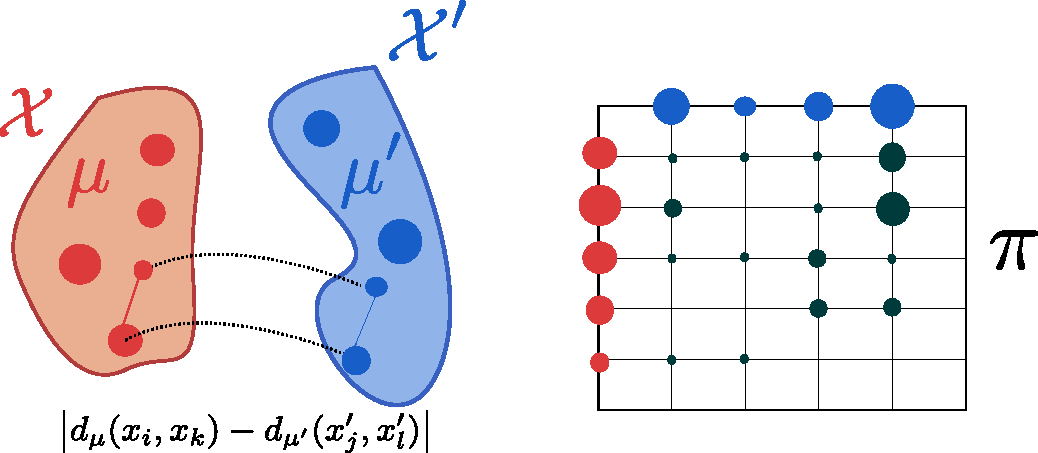
\includegraphics[width=.6\textwidth]{fig/gw}
\caption{Gromov-Wasserstein distance. \label{fig:gw}}
\end{figure}

The corresponding distance is the Gromov-Wasserstein distance, defined as:

\begin{equation}
    GW_p(\mu, \mu') = \min_{\pi \in \Pi(\mu, \mu^\prime)}
        \left(
            \sum_{i,j,k,l}
            \left| d_\mu(x_i, x_k) - d_{\mu'}(x^\prime_j, x^\prime_l) \right|^p
            \pi_{i,j} \pi_{k,l}
        \right)^{\frac{1}{p}}
    \label{eq:gw}
\end{equation}

where $d_\mu$ (resp. $d_{\mu'}$) is the metric associated to $\mathcal{X}$
(resp. $\mathcal{X}^\prime$), the space in which $\mu$ (resp. $\mu'$) lies.

\subsection{Sliced Gromov-Wasserstein}

Computational complexity associated to the optimization problem in
Equation \eqref{eq:gw} is high in general.
However, we have shown in~\cite{vayer:hal-02174309} that in the
mono-dimensional case, this problem can be seen as an instance of the Quadratic
Assignment Problem~\cite{koopmans1957assignment}.
We have provided a closed form solution for this instance.
In a nutshell, our solution consists in sorting mono-dimensional distributions
and either matching elements from both distributions in order or in reverse
order, leading to a $O(n \log n)$ algorithm that exactly solves this problem.

Based on this closed-form solution, we were able to introduce a Sliced
Gromov-Wasserstein distance that, similarly to the Sliced Wasserstein
distance~\cite{rabin2011wasserstein}, computes similarity between distributions
through projections on random lines.

\todo{TODO: add a summary of Titouan's last findings about GW when they are
stabilized.}

\subsection{Fused Gromov-Wasserstein}

Here, we focus on comparing structured data which combine a feature
and a structure information.
More formally, we consider undirected labeled graphs as tuples of the form $\mathcal{G}=(\mathcal{V},\mathcal{E},\ell_f,\ell_s)$ where
$(\mathcal{V},\mathcal{E})$ are the set of vertices and edges of the graph.
$\ell_f: \mathcal{V} \rightarrow \Omega_f$ is a labelling function which
associates each vertex $v_{i} \in \mathcal{V}$ with a feature
$a_{i} = \ell_f(v_{i})$ in some feature metric space
$(\Omega_f,d)$.
We will denote by \emph{feature information} the set of all the features
$\{a_{i}\}_{i}$ of the graph.
Similarly, $\ell_s: \mathcal{V} \rightarrow \Omega_s$ maps a vertex $v_i$ from
the graph to its structure representation
$x_{i} = \ell_s(v_{i})$ in some structure space
$(\Omega_s,C)$ specific to each graph.
$C : \Omega_s \times \Omega_s \rightarrow \mathbb{R_{+}}$ is a symmetric
application which aims at measuring the similarity between the nodes in the
graph.
Unlike the feature space however, $\Omega_s$ is implicit and in practice,
knowing the similarity measure $C$ will be sufficient. With a slight abuse of
notation, $C$ will be used in the following to denote both the structure
similarity measure and the matrix that encodes this similarity between pairs of
nodes in the graph $\{C(i,k) = C(x_i, x_k)\}_{i,k}$.
Depending on the context, $C$ can either encode the neighborhood information of
the nodes, the edge information of the graph or more generally it can model a
distance between the nodes such as the shortest path distance.
When $C$ is a metric, such as the shortest-path
distance, we naturally endow the structure with the metric space $(\Omega_s,C)$.
We will denote by \emph{structure information} the set of all the structure
embeddings $\{x_{i}\}_i$ of the graph.
We propose to enrich the previously described graph with a histogram which
serves the purpose of signaling the relative importance of the vertices in the
graph.
To do so, we equip graph vertices with weights $\{h_{i}\}_{i}$ that sum to $1$.

All in all, we define \emph{structured data} as a
tuple $\mathcal{S}=(\mathcal{G},h_{\mathcal{G}})$ where $\mathcal{G}$ is a
graph as described previously and $h_{\mathcal{G}}$ is a function that
associates a weight to each vertex. This definition allows the graph to be
represented by a fully supported probability measure over the product space
feature/structure $\mu= \sum_{i=1}^{n} h_{i} \delta_{(x_{i},a_{i})}$ which
describes the entire structured data, as shown in Figure~\ref{fig:graph}.

\begin{figure}
\centering
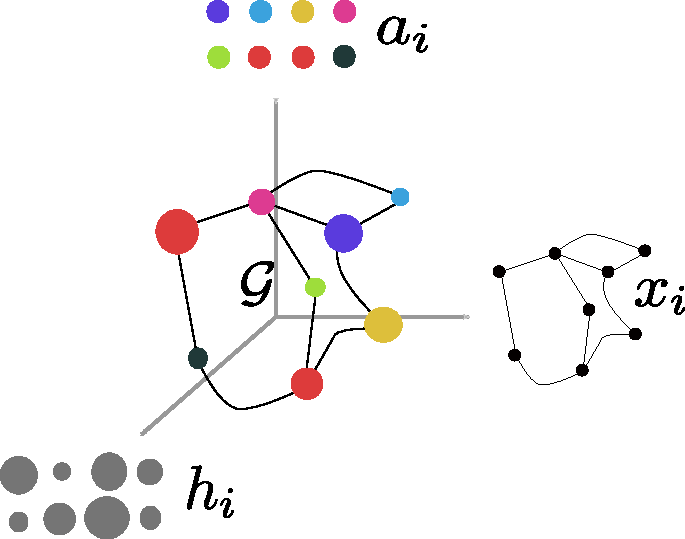
\includegraphics[width=.4\textwidth]{fig/graph_as_distrib}
\caption{Structured object can be described by a labelled graph with $(a_{i})_{i}$ the feature information of the object and $(x_{i})_{i}$ the structure information.
If we enrich this object with a histrogram $(h_{i})_{i}$ aiming at measuring the relative importance of the nodes between them we can represent the structured object as a fully supported probability measure $\mu$ over the couple space of feature and structure. \label{fig:graph}}
\end{figure}

\subsubsection{Distance definition and properties}

Let $\mathcal{G}$ and $\mathcal{G}'$ be two graphs, described respectively
by their probability measure $\mu= \sum_{i=1}^{n} h_{i} \delta_{(x_{i},a_{i})}$
and $\mu' = \sum_{i=1}^{m} h^\prime_i \delta_{(x^\prime_i,a^\prime_i)}$.
Their structure matrices are denoted $C$ and $C'$, respectively.


We define a novel Optimal Transport discrepancy called the
Fused Gromov-Wasserstein distance.
It is defined, for a trade-off parameter  $\alpha \in [0,1]$, as

\begin{equation}
\label{discretefgw}
FGW_{q, \alpha} (\mu, \mu') = \min_{\pi \in \Pi(\mu, \mu^\prime)}
    E_{q}(\mathcal{G}, \mathcal{G}', \pi)
\end{equation}

where $\pi$ is a transport map (\emph{i.e.} it has marginals $h$ and $h'$) and

\begin{equation}
E_{q}(\mathcal{G}, \mathcal{G}', \pi) =
    \sum_{i,j,k,l} (1-\alpha) d(a_{i},a^\prime_j)^{q}
                    +\alpha |C(i,k)-C'(j,l)|^{q} \pi_{i,j}\pi_{k,l} .
\end{equation}

The FGW distance looks for the coupling $\pi$ between vertices of the
graphs that minimizes the cost $E_{q}$ which is a linear combination of a cost
$d(a_{i},a^\prime_j)$ of transporting feature $a_{i}$ to $a^\prime_j$
and a cost $|C(i,k)-C'(j,l)|$ of transporting pairs of nodes in each structure.
As such, the optimal coupling tends to associate pairs of feature and
structure points with similar distances within each structure pair and with
similar features.
As an important feature of FGW, by relying on a sum of
(inter- and intra-)vertex-to-vertex distances, it can handle structured data
with continuous attributed or discrete labeled nodes
(depending on the definition of $d$) and can also be computed even if the graphs
have different numbers of nodes.

We have shown in~\cite{vayer:hal-02174322} that FGW retains the following
properties:

\begin{itemize}
\item it defines a metric for $q=1$ and a semi-metric for $q >1$;
\item varying $\alpha$ between 0 and 1 allows to interpolate between the
Wasserstein distance between the features and the Gromov-Wasserstein distance
between the structures;
\end{itemize}

We also define a continuous counterpart for FGW which comes with a
concentration inequality in~\cite{vayer:hal-02174316}.
We present a Conditional Gradient algorithm for optimization on the
above-defined loss.
We also provide a Block Coordinate Descent algorithm to compute graph
barycenters \emph{w.r.t.} FGW, such as the ones presented in
Figure~\ref{fig:bary_fgw}.

\subsubsection{Results}

\begin{figure}
\centering
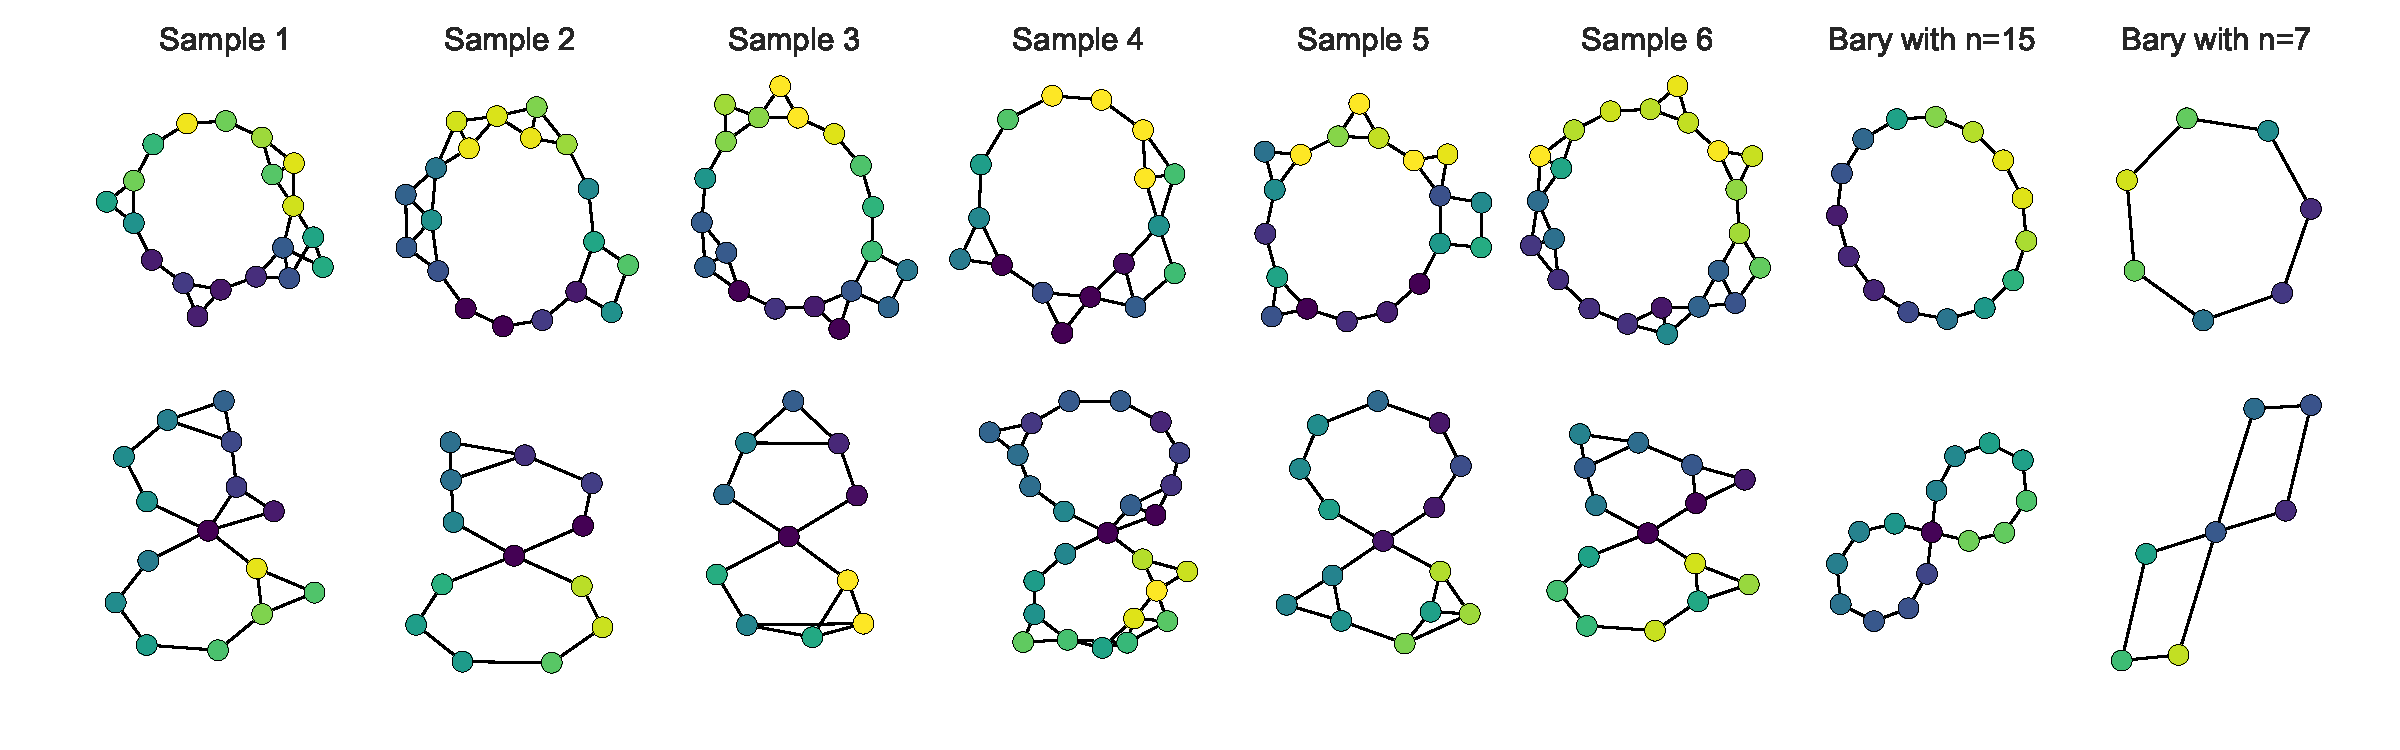
\includegraphics[width=\textwidth]{fig/fgw_bary}
\caption{Example barycenters computed using FGW as a metric for two datasets of
noisy labeled graphs. \label{fig:bary_fgw}}
\end{figure}

We have shown that FGW allows to extract meaningful barycenters, as presented
in Figure~\ref{fig:bary_fgw}.
These barycenters can be used for graph clustering.
Finally, we have exhibited classification results for FGW embedded in a
Gaussian kernel SVM which leads to state-of-the-art performance
(even outperforming graph
neural network approaches) on a wide range of graph classification problems.

